% !TEX root = dokumentation.tex
\section{Implementierung}\label{sec:impl}
In diesem Kapitel wird die konkrete Entwicklung des Spieles beschrieben. Dabei werden sowohl die verschiedenen Prototypen betrachtet, wichtige Design-Entscheidungen offen gelegt und die technischen Hintergründe erläutert.
\subsection{Prototypeing}
	Als Basis der Implementierung wird ein in Unity vorhandenes Beispiel verwendet\footnote{<TODO:paket nennen>}, welches im Lauf der Entwicklung entsprechend angepasst und erweitert wird. Zu diesem Beispiel gehört ein vereinfachtes Modell eines Autos, eine Kamera, welche sich hinter dem Fahrzeug befindet und einfache Nutzersteuerung für die Tastatur.
	In diesem Abschnitt der Studienarbeit sollen nun die Prototypen in chronologischer Reihenfolge dargestellt werden, um die Entwicklung des Spiels zu verdeutlichen. Alle Stadien des Spiels werden sowohl von den Entwicklern, wie auch ausgewählten Testspielern geprüft. Das erhaltene Feedback bietet somit die maßgebliche Grundlage für die Änderungen zwischen zwei Prototypen. Eine ausführliche Darlegung der Design-Entscheidungen befindet sich im folgenden Kapitel.
	\begin{enumerate}[label=Prototyp \arabic*]
		\item{ Für den Beginn der Entwicklung wird zunächst eine Kopie des genannten Beispieles angefertigt. Auf Basis der grundsätzlichen Spielidee wird die Kamera oberhalb des Fahrzeugs positioniert, um eine Top-Down Ansicht zu erhalten. Durch die initiale Positionierung der Kamera hinter dem Fahrzeug, rotiert die Kamera mit dem Fahrzeug. Zwecks besserer Übersichtlichkeit wird dieses Drehverhalten unterbunden und die Kamera lediglich relativ zur Position, jedoch nicht der Rotation des Fahrzeugs erweitert. Um das Spiel auf mobilen Endgeräten spielen zu können, ist eine zunächst vereinfachte Steuerung über einen Joystick und zwei Buttons, vorwärts und rückwärts, nötig. Die Eingaben des Joysticks werden relativ zur Rotation des Fahrzeugs verarbeitet, somit führt beispielsweise ein \enquote{nach links ziehen} des Joysticks zu einer Linkskurve des Fahrzeugs. Die vertikale Achse des Joysticks findet in diesem Prototyp keine Verwendung. }
		\item{ Für den zweiten Prototyp steht die Weiterentwicklung der Steuerung im Fokus. Für eine neue Umsetzung der Steuerung wird sowohl die horizontale, wie auch die vertikale Achse benötigt. Anschließend wird die Steuerung nicht relativ zur Ausrichtung des Fahrzeugs, sondern relativ zur Blickrichtung der Kamera implementiert. Somit schlägt das Fahrzeug immer die gleiche Richtung ein, wie der Joystick abhängig von seinem Mittelpunkt bewegt wird. Ein Ziehen des Joysticks nach rechts führt somit in jedem Fall dazu, dass das Fahrzeug nach rechts fährt. Die vorherige Fahrtrichtung des Fahrzeugs spielt dabei keine Rolle. }
		\item{ Auch der dritte Prototyp des Spiels hat die grundsätzliche Steuerung zum Ziel. Auf Basis mehrerer erhaltenen Kritiken soll das Verhalten des \enquote{Rückwärts-Pedals} verändert werden. Hauptkritikpunkt in diesem Fall ist, dass ein reales Fahrzeug kein eigens Pedal für den Rückwärtsgang besitzt. Mit einer Veränderung dieses Steuerungselements verändert sich das Rückwärts-Pedal zu einem Bremspedal. Ein Betätigen dieser Schaltfläche reduziert die Fahrtgeschwindigkeit bis zum Stillstand. Dem somit fehlende Rückwärtsgang wird zunächst keine Beachtung geschenkt, dies soll mit einem späteren Prototyp implementiert werden.}
		\item{ Um die Optik des Spiels aufzuwerten, steht für den vierten Prototyp die Benutzeroberfläche im Fokus. Dabei werden sowohl für alle Buttons, wie auch für den Joystick eigene Grafiken erstellt. Alle Grafiken der Benutzerobefläche folgen dem gleichen Konzept und vermitteln somit ein wohl überlegtes Gesamtbild. Für die Gestaltung der Buttons für Gas und Bremse wird eine Evaluation durchgeführt. Der vorläufige Gewinner dieser Evaluation sind zwei Tachos, wobei ein Tacho einen hohen Wert und ein Tacho einen niedrigen Wert anzeigt. }
		\item{ Mit dem fünften Prototyp kann der Rückwärtsgang implementiert werden. Ein \enquote{nach Hinten ziehen} des Joysticks führt dabei zu einer Änderung der Fahrtrichtung des Fahrzeugs. Bei der Beschleunigung fährt das Fahrzeug somit rückwärts. Auch die Steuerung wird in diesem Fall so invertiert, dass das Fahrzeug weiterhin der Ausrichtung des Joysticks folgt. Weiterhin wird während dieses Prototyps ein Anzeigen der Aufgaben möglich gemacht. Das Durchfahren eines bestimmten Bereichs führt dazu, dass auf dem Bildschirm eine zufällige Aufgabe aus der Liste aller möglichen Aufgaben gewählt wird. Die möglichen Lösungen dieser Aufgabe werden zu diesem Zeitpunkt noch nicht angezeigt. Zusätzlich zu den Änderungen an der Spielmechanik existiert seit diesem Prototyp eine Minimap, welche dem Spieler den kommenden Streckenverlauf transparent auf dem Bildschirm anzeigt. }
		\item{ Die Finalisierung der Aufgaben innerhalb der Level ist der Kernaspekt des sechsten Prototyps. Dabei werden zunächst neben der Aufgabe auch zwei mögliche Lösungen dieser Aufgabe angezeigt. Die Lösungen der Aufgaben sind entweder in blau oder in rot eingefärbt, welche Farbe für die richtige Lösung verwendet wird ist dabei zufällig gewählt. In den einzelnen Rennen werden den existierenden Weggabelungen Pfeile hinzugefügt, welche in den Farben der Aufgaben eingefärbt sind. Somit sieht der Spieler unmittelbar, welcher Weg zu welcher möglichen Lösung gehört. Zudem wird bei Durchfahren der Wege ausgewertet, ob die Aufgabe korrekt oder inkorrekt gelöst ist. }
		\item{ Die siebte Version des Spiels stellt die Fertigstellung der Fahrzeugsteuerung dar. Der Wechsel zwischen dem Vorwärtsgang und dem Rückwärtsgang soll nur möglich sein, wenn das Fahrzeug still steht. Durch diese Änderung führt ein \enquote{Verreißen} des Joysticks lediglich zu einer Richtungsänderung, jedoch nicht mehr zum apprupten Abbremsen des Fahrzeugs. Da die generelle Steuerung als \enquote{zu empfindlich} kritisiert wird, wird eine Lenkungsverzögerung implementiert. An diesem Punkt erreicht die Steuerung den finalen Status.}
		\item{ Um eine globale Verfügbarkeit der Spieler-Daten über ein Schließen der App heraus zu gewährleisten, wird eine Speicherung des Spielstands implementiert. In diesem Spielstand ist gespeichert, welche Rennen ein Nutzer bereits abgeschlossen hat, welche Finalrennen bereits freigespielt sind, wieviele Münzen der Spieler besitzt und wieviele Aufgaben bereits erfolgreich gelöst sind. Über die Anzahl der Aufgaben ist eine Statistik über den Lernerfolg des Spielers möglich, wird jedoch in diesem Fall nicht realisiert. Weiterhin erhalten die einzelnen Rennen eine Auswertung darüber, ob ein Rennen gewonnen ist, oder nicht. Die genauen Kriterien für das Gewinnen eines Rennens befinden sich im folgenden Kapitel. Durch die nun verfügbaren Informationen über die Anzahl an Münzen ist die Einführung des Ingame-Shops möglich. Dieser ist als eigenes Level realisiert und über Startmenü des Spiels erreichbar.}
		\item{ Damit das Spiel auch multilingual nutzbar ist, sollen jegliche Texte durch Symbole ersetzt werden. Weitere Symbole, welche dem gleichen Konzept wie bisherige Buttons folgen werden entworfen und umgesetzt. Mit dem Einbau dieser Symbole im Spiel sind jegliche Texte im Spiel nicht mehr nötig. Somit ist das Spiel grundsätzlich universal einsetzbar, die Sprache der Spieler ist irrelevant. Um die Dynamik und das Spielgefühl zu verbessern, werden dem Spiel verschiedene Töne hinzugefügt. So wird beispielsweise ein korrektes Lösen einer Aufgabe mit Jubel belohnt. Eine Kollision mit Objekten der Karte verursacht nun ebenso Geräusche. Zusätzlich erhält das Spiel Hintergrundtöne, welche die Spielwelt lebendiger wirken lassen. Mit der Fertigstellung dieses Prototyps ist die gewünschte Grundfunktionalität erreicht. Alle weiteren Schritte in der Entwicklung führen zu weiteren Levelpacks und spielbaren Leveln.}
	\end{enumerate}
\subsection{Design-Entscheidungen in der Entwicklung}
In diesem Kapitel sollen während des Prototypings aufgetretene Designentscheidungen aufgegriffen und erläutert werden. Dabei werden die Argumente sowie Meinungen von Testspielern einbezogen.
	\subsubsection{Automatische Beschleunigung vs Gaspedal}
	Kern dieser Entscheidung ist die Frage, ob der Nutzer einen Button betätigen muss, damit sein Fahrzeug fährt. Als Automatisches Gas sind hierbei zwei Interpretationen möglich:
	\begin{itemize}
	\item{ Das Fahrzeug beschleunigt vollständig automatisch und der Nutzer lenkt lediglich die Fahrtrichtung.}
	\item{ Das Fahrzeug beginnt zu beschleunigen, sobald der Nutzer den Joystick bewegt. Der Joystick bestimmt somit sowohl die Fahrtrichtung, als auch die Geschwindigkeit.}
	\end{itemize}
	Bei einer vollständig automatischen Beschleunigung wäre für die Steuerung lediglich eine Schaltfläche nötig, welche für das Bremsen des Fahrzeugs zuständig ist. Eine Implementierung des Rückwärtsgangs ist an dieser Stelle schwierig, da ein spontaner Wechsel der Fahrtrichtung einer Invertierung des Beschleunigungsvektors entspricht. Zusätzlich hat der Spieler weniger Möglichkeiten, die Geschwindigkeit des Fahrzeugs an die Streckenverhältnisse anzupassen. Wird die Beschleunigung über den Joystick reguliert, entfällt das Problem des Rückwärtsgangs, die fehlende Anpassungsmöglichkeit der Geschwindigkeit bleibt jedoch bestehen.
	Wird dem Nutzer eine Schaltfläche für die Beschleunigung geboten, so hat dieser die Möglichkeit, die Geschwindigkeit zu verringern ohne das Bremspedal betätigen zu müssen. Somit kann die Geschwindigkeit des Fahrzeugs optimal an die Straßenverhältnisse angepasst werden. Aus diesem Grund wird von einer Implementierung einer automatischen Beschleunigung abgesehen.

	\subsubsection{Steuerung relativ zu Kamera vs Steuerung relativ zu Fahrzeug}
    Die Wahl der Verankerung der Steuerung kann gravierende Änderungen an dem Spielerlebnis des Nutzers haben. Aus diesem Grund ist diese Entscheidung sehr wichtig und muss genau analysiert werden.
    Wird die Steuerung relativ zur Ausrichtung der Kamera implementiert, so reagiert das Fahrzeug jederzeit mit einer Rotation in Richtung der Ausrichtung des Joysticks. Zieht der Anwender den Joystick beispielsweise nach rechts, so bewegt sich das Fahrzeug jederzeit in Richtung des rechten Bildschirmrands. Bei der Steuerung relativ zur Ausrichtung des Fahrzeugs ist diese Kontinuität nicht gegeben. Fährt das Fahrzeug aus Sicht des Nutzers nach oben, so führt ein nach rechts ziehen des Joysticks zu einer Rechtskurve und somit einer Richtungsänderung nach rechts.
    Fährt das Fahrzeug jedoch aus der Sicht des Nutzers nach unten, so führt ein nach rechts ziehen des Joysticks zwar ebenfalls zu einer Rechtskurve, jedoch entspricht dies auf Basis der vorherigen Fahrtrichtung einer Änderung der Fahrtrichtung nach links.
    Bei der Steuerung relativ zur Position des Fahrzeugs bedeutet dies, dass stetig Transferleistungen erbracht werden müssen. Der Spieler muss sich jederzeit überlegen, wie das Fahrzeug seine Eingabe verarbeitet. Da dies bei einer Steuerung relativ zur Kamera nicht der Fall ist, kann diese Möglichkeit allgemein als \enquote{einfacher} gewertet werden. Da die Zielgruppe des Spiels vor allem Kinder im Grundschulalter sind, ist die einfachere Steuerung zu bevorzugen. Ein weiterer Pluspunkt der Steuerung relativ zur Kamera ist die Präzision. Da das Fahrzeug jederzeit die Fahrtrichtung des Joysticks übernimmt, kann das Fahrzeug sehr präzise gesteuert werden.

	\subsubsection{Implementierung des Rückwärtsgangs}
	Für die Implementierung des Rückwärtsgangs stehen grundsätzlich zwei Möglichkeiten zur Auswahl.
	\begin{itemize}
		\item{ Das Bremspedal erfüllt gleichzeitig die Funktion, das Fahrzeug zu verlangsamen, sowie ab Erreichen des Stillstands entgegen der Fahrtrichtung zu beschleunigen.}
		\item{ Die Ausrichtung des Joysticks bestimmt die Wahl der Fahrtrichtung. Wird der Joystick entgegen der Ausrichtung bewegt, fährt das Fahrzeug rückwärts.}
	\end{itemize}
	Erfüllt das Bremspedal die Funktion, das Fahrzeug rückwärts zu beschleunigen, so verliert das Spiel an Konsistenz. In diesem Fall wechseln die beiden Pedale ihre Funktionalität. Bewegt sich das Fahrzeug nach vorn, so dient das Bremspedal zur Verlangsamung des Fahrzeugs. Bewegt sich das Fahrzeug hingegen bereits rückwärts, so führt ein Betätigen des \enquote{Bremspedals} zu einer Erhöhung der Fahrtgeschwindigkeit in die Rückwärts-Richtung. In diesem Fall muss der Nutzer das \enquote{Gaspedal} betätigen, um das Fahrzeug zu verlangsamen und im Endeffekt die Fahrtrichtung erneut auf Vorwärts zu wechseln.
	Wird die Ausrichtung des Joysticks zur Wahl der Fahrtrichtung verwendet, so wird die Konsistenz gewahrt. Das Betätigen des Bremspedals führt dabei ungeachtet der Fahrtrichtung zu einer Verlangsamung des Fahrzeugs, wohingegen ein Betätigen des Gaspedals in jedem Fall zu einer Beschleunigung des Fahrzeugs führt. Da die Wahrung der Konsistenz für die Entwicklung eines Spiels eine große Rolle spielt, wird für die Implementierung des Rückwärtsgangs die Abhängigkeit zur Ausrichtung des Joysticks gewählt.

	\subsubsection{Auswertung eines Rennens}
	Für die Auswertung eines Rennens und somit für die Vergabe der Pokale und Punkte wird  eine Entscheidungstabelle hergeleitet. Die dafür relevanten Kriterien sind die Prozentzahl der korrekten Aufgaben und die Zeit, welche der Spieler für die Strecke benötigt hat.
	Für die Auswertung der benötigten Zeit erhält jedes Level drei Zeiten, welche zur Bestimmung der Rennleistung genutzt werden. Für jede dieser Zeiten existieren zwei Stadien und für die schnellste und langsamste Zeit je ein zusätzliches:
	\begin{enumerate}
		\item{ Langsamer als die gesetzte Zeit, jedoch näher an dieser, als an der nächst langsameren Zeit. Für die letzte Zeit wird hier ein maximal Abstand von $60$ Sekunden verwendet. Alles darunter ist \enquote{zu langsam} und in der folgenden Tabelle mit $<<$ markiert. }
		\item{ Schneller als die jeweilige Zeit, dabei jedoch nicht näher an der nächst schnelleren Zeit. Für die Erste beziehungsweise schnellste Zeit wird diese Gruppe mit $60$ Sekunden Differenz definiert. Schnellere Zeiten sind unter $>>$ zusammengefasst. }
	\end{enumerate}
	Wie in \ref{gewinnbedinungen} definiert soll ebenso die Menge der korrekten Aufgaben in die Gewinnfunktion einfließen. Die Aufgaben werden in 4 Regionen unterteilt:
	\begin{enumerate}
		\item{ unter 30\% der Aufgaben wurden korrekt gelöst. }
		\item{ unter 60\% der Aufgaben wurden korrekt gelöst. }
		\item{ unter 100\% der Aufgaben wurden korrekt gelöst. }
		\item{ 100\% der Aufgaben wurden korrekt gelöst. }
	\end{enumerate}
	Mit diesen beiden Achsen kann so die folgende Tabelle mit den jeweiligen gewonnenen Pokalen definiert werden:

	\newcommand{\bronze}{\raisebox{-.5ex}{
\includegraphics[height=12pt]{img/pokal_bronze.pdf}}}
	\newcommand{\silber}{\raisebox{-.5ex}{
\includegraphics[height=12pt]{img/pokal_silber.pdf}}}
	\newcommand{\gold}{\raisebox{-.5ex}{
\includegraphics[height=12pt]{img/pokal_gold.pdf}}}
	\begin{tabl}{r@{\hspace{8mm}}cccrlccc}{Vergabe von Pokalen}%
		\toprule\label{pokal-tabelle}
			& \multicolumn{3}{c}{Dritte Zeit} & \multicolumn{2}{c}{Zweite Zeit} & \multicolumn{3}{c}{Erste Zeit} \\
			$\sum$ Aufgaben & $<<$ & $<$ & $>$ & $<$ & $>$ & $<$ & $>$ & $>>$ \\
		\midrule
			$<30\%$ & $-$ & $-$ & $-$ & \hspace{5mm}$-$ & $-$\hspace{4mm} & $-$ & $-$ & \bronze \\
			$<60\%$ & $-$ & \bronze & \bronze & \bronze & \bronze & \bronze & \silber & \silber \\
			$<100\%$ & $-$ & \bronze & \bronze & \bronze & \silber & \silber & \silber & \silber \\
			$=100\%$ & $-$ & \bronze & \silber & \silber & \silber & \silber & \gold & \gold \\
		\bottomrule
	\end{tabl}

Das Erreichen von Gold-Pokalen wird dabei absichtlich schwierig gewählt, um den Spieler zu fordern, motivieren und auch um realistische Ergebnisse zu setzen. Erst wenn die Aufgaben und die Zeit perfektioniert wurden, erhält der Spieler einen Gold-Pokal.
Mit dieser Entscheidungstabelle ist der Grad zwischen Spielern, welche sehr gut Rennen fahren können, und Spielern, welche gut im Lösen der Aufgaben sind, perfekt ausgeglichen. Ein Spieler kann das Rennen schaffen (beziehungsweise einen Bronze-Pokal erhalten), ohne eine Aufgabe korrekt zu lösen. Allerdings muss die gespielte Zeit dabei die schnellste Zeit deutlich unterschreiten, was einem perfekt gefahrenen Rennen ohne Fehler gleichkommt. Andererseits kann beispielsweise ein Silber-Pokal bereits erreicht werden, wenn der Spieler schneller als die langsamste Zeit fährt und alle Aufgaben korrekt löst.

\subsection{Entwicklungsablauf in Unity}
Bei der Entwicklung von Anwendungen mit Unity erhält der Anwender mehrere Möglichkeiten zur Verfügung. In diesem Kapitel sollen die Kompontenen von Unity, welche bei der Entwicklung des Spiels verwendet werden, beleuchtet werden.

\subsubsection{Scene View}
\figur{Unity-SceneView.png}{\label{ssec:sceneView}Die Unity Scene View mit Hierarchy Reiter}
Die Unity Scene View ist der Leveleditor von Unity. In der Scene View kann der Nutzer (abhängig vom verwendeten Modus) 2D oder 3D Objekte im Level platzieren. Jegliche (optische) Gestaltung der einzelnen Level, genauso wie die Erstellung des User Interface oder das Platzieren von Kollisionszonen findet in der Scene View statt. Über den Hierarchy Reiter kann der Anwender alle im Level platzierten Objekte auswählen, um beispielsweise deren Position in der Scene View zu ändern. 


\subsection{Entwicklung}
In diesem Kapitel der Arbeit werden wichtige Schritte in der Entwicklung der Anwendung aufgegriffen. Dabei liegt der Fokus besonders auf Kernaspekten bzw. Kernproblemen, welche im Laufe der Entwicklung aufkommen.
	\subsubsection{Level Design}
		Wie bereits in \ref{par:streckendesign} und \ref{par:streckendesign2} beschrieben sollen die Rennstrecken schlauchartig aufgebaut sein. Das bedeutet, dass für jedes Level ein fester Startpunkt sowie ein fester Endpunkt existiert. Weiterhin existiert nur ein korrekter Weg zwischen diesen Punkten. Grundsätzlich können dem Spieler Abzweigungen innerhalb des Levels angeboten werden, diese Abzweigungen führen den Spieler jedoch nicht ans Ziel. 
		\figur{Schlauchlevel.png}{\label{ssec:schlauch}Beispiel: Schlauchlevel}
		Die Abbildung \ref{ssec:schlauch} zeigt einen Ausschnitt eines Levels. In der Mitte der Abbildung befindet sich die Rennstrecke, welche auf beiden Seiten von einem Seitenstreifen eingeschlossen wird. An den Außenrändern der Seitenstreifen befinden sich statische Objekte, welche ein Verlassen des vorgegeben Wegs verhindern. Somit wird gewährleistet, dass der Spieler den vorgegeben Bereich nicht verlassen kann und ungewollte Abkürzungen zwischen dem Start und dem Ziel nicht existieren. Durch die Entscheidung für Schlauchlevel kann dem Spieler ein klar vorgegebener Rahmen präsentiert werden. Der Bereich außerhalb dieses Schlauches kann aus den genannten Gründen im Bereich des Leveldesigns ignoriert werden. Verlässt der Spieler den in der Abbildung \ref{ssec:schlauch} braun markierten Bereich, wird ein C\# Script ausgelöst, welches die Geschwindigkeit verringert. Die genaue Umsetzung der Geschwindigkeitsreduktion soll an dieser Stelle nicht behandelt werden. Nähere Informationen dazu befinden sich im Kapitel <TODO: Verlinkung einfügen>.
		\figur{Statische_Objekte.png}{\label{ssec:statisch}Beispiel: Unbewegliche Objekte neben der Strecke}
		Wie in der Abbildung \ref{ssec:statisch} zu sehen ist, befinden sich sowohl rechts und links der Straße Gebäude oder ähnliche Gegenstände. In der Abbildung zu sehen sind beispielsweise zwei Häuser, ein Brunnen, ein Sonnensegel sowie ein großer, runder Stein. Weitere Objekte, welche sich neben der Strecke befinden können sind abhängig von den jeweiligen Levelpacks. In den Wald-Leveln können beispielsweise Bäume, Baumstümpfe, Felsen, Zäune das befahren der Seitenstreifen erschweren. Im zweiten implementierten Levelpack, welches an einen stillgelegten Kanal angelehnt ist, können beispielsweise Treppen, tiefe Pfützen oder auch Brückenpfeiler die Seitenstreifen blockieren. Diese Objekte sind unbeweglich, eine Kollision des Fahrzeugs mit diesen Objekten führt (abhängig vom Winkel der Kollision) zu einem Stillstand des Fahrzeugs. Um den Spielfluss nicht maßgeblich zu beeinträchtigen, sind diese Objekte ausschließlich neben der eigentlichen Strecke platziert. Somit kann eine Kollision verhindert werden, indem die Strecke nicht verlassen wird. 
		\figur{Bewegliche_Objekte.png}{\label{ssec:beweglich}Beispiel: Bewegliche Objekte auf der Strecke}
		Wie in \ref{par:streckendesign2} erwähnt, werden auch bewegliche Objekte in den Leveln verwendet. Die Abbildung \ref{ssec:beweglich} zeigt einen Ausschnitt aus dem zweiten Levelpack. Auf der Strecke befinden sich bewegliche Fässer und Leitkegel. Zusätzlich sind zwei Pfützen zu sehen, welche das Fahrzeug beim Durchfahren bremsen. Die Fässer und Leitgekel sind mit physikalischen Eigenschaften (sogenannten \enquote{Rigid Bodys}) ausgestattet. Über diese Eigenschaften kann ein Gewicht für das Objekt festgelegt werden. In Kombination mit dem Gewicht des Fahrzeugs und dessen Geschwindigkeit wird das Objekt bei einer Kollision weggestoßen. Weitere denkbare bewegliche Objekte können beispielsweise Reifenstapel, kleinere Steine oder Warnbarken sein. 
		Der letzte Aspekt, welcher im Rahmen des Level Designs betrachtet werden soll, ist die Realisierung der Aufgaben. Wie in \ref{par:aufgaben} bereits erwähnt, erhält der Spieler eine Aufgabe und zwei potentielle Lösungen auf dem Bildschirm angezeigt. Somit ist für das Level Design eine Realisierung einer Auswahlmöglichkeit zwischen diesen beiden Lösungen notwendig. Die Implementierung dieser Auswahlmöglichkeit unterscheidet sich hierbei abhängig vom ausgewählten Levelpaket. 
		\figur{Roadsplit.png}{\label{ssec:roadsplit}Beispiel: Aufspaltung der Straße}
		Die Abbildung \ref{ssec:roadsplit} entstammt dem ersten Levelpaket. Sie zeigt die Stelle der Auswertung der Aufgaben. An dieser Stelle teilt sich die Strecke in zwei mögliche Wege. Die beiden Wege sind exakt gleich lang. Dabei ist einer der beiden Wege mit der korrekten, der jeweils andere Weg mit der falschen Lösung assoziiert. Die Verteilung, welcher der beiden Wege die korrekte Lösung erhält, geschieht zufällig. 
		\figur{Split-Tunnel.png}{\label{ssec:tunnel}Beispiel: Zwei mögliche Tunnel}
		Im zweiten Levelpack wird auf ein Aufspalten der Strecke verzichtet. Im Fall der Abbildung \ref{ssec:tunnel} ist die Entscheidung auf einen Tunnel mit zwei Eingängen gefallen. Dabei ist ebenso ein Eingang mit der korrekten, und ein Eingang mit der falschen Lösung verbunden. In beiden Levelpaketen wird der Nutzer durch farbige Pfeile auf der Strecke (vgl. Abbildung \ref{ssec:roadsplit} und Abbildung \ref{ssec:tunnel}) darauf hingewiesen, welche Lösung zu welchem möglichen Weg gehört. 

	\subsubsection{UI Design}
	In frühen Versionen des Spiels sind wichtige Funktionen für die Interaktion mit dem Nutzer durch beschriftete Buttons realisiert. Um eine multilinguale Einsetzbarkeit des Spiels zu gewährleisten, werden diese Beschriftungen aus dem Spiel entfernt und durch aussagekräftige Icons ersetzt.	Für die Entwicklung eines User Interfaces steht zunächst ein einheitliches Layout im Vordergrund. Dabei wird besonderes Augenmerk auf gleichbleibende Skalierung sowie ein einheitliches Design der Icons für das Spiel geachtet.
	\figur{icons.pdf}{\label{ssec:buttons}Übersicht über Icons}
	Die Abblidung \ref{ssec:buttons} zeigt einen Überblick über die im Spiel verwendeten Symbole. Für jede wichtige Interaktionsmöglichkeit des Nutzers mit der Anwendung existiert ein zugehöriges Symbol:
	\begin{itemize}
		\item{ Zur Steuerung des Fahrzeugs wird ein Joystick mit Pfeilen verwendet.}
		\item{ Über zwei Pedale kann das Fahrzeug beschleunigt und abgebremst werden. Die Pedale sind dabei mit Größenverhältnis und Form an reale Fahrzeugpedale angepasst.}
		\item{ Durch Betätigen des runden Pfeils kann das Rennen neu gestartet werden.}
		\item{ Das Zahnrad öffnet das Optionsmenü des Spiels.}
		\item{ Der Pause- und Play-Button pausieren das Rennen und setzen es fort.}
		\item{ Das Haus-Symbol bringt den Spieler zurück ins Hauptmenü.}
		\item{ Das Haken-Symbol wird im Shop verwendet und bestätigt einen Kauf.}
	\end{itemize}
	Bei allen erwähnten Symbolen wird ein gleichbleibender Farbverlauf verwendet. Außerdem sind alle Icons mit einem helleren Rand versehen. 
	Eine Besonderheit stellt die Visualisierung der beiden Pedale dar. In der Abbildung \ref{ssec:buttons} sind lediglich die final gewählten Designs enthalten. Für die Darstellung der beiden Funktionen \enquote{Gas geben} und \enquote{Bremsen} als Icons sind im Laufe der Entwicklung viele Zwischenstadien entstanden. Die wichtigsten dieser Zwischenstadien zeigt die Tabelle. Die entsprechenden Kritiken und Erläuterungen können der folgenden Tabelle entnommen werden. 
	\newcommand{\pedaleSchrift}{\raisebox{-.5ex}{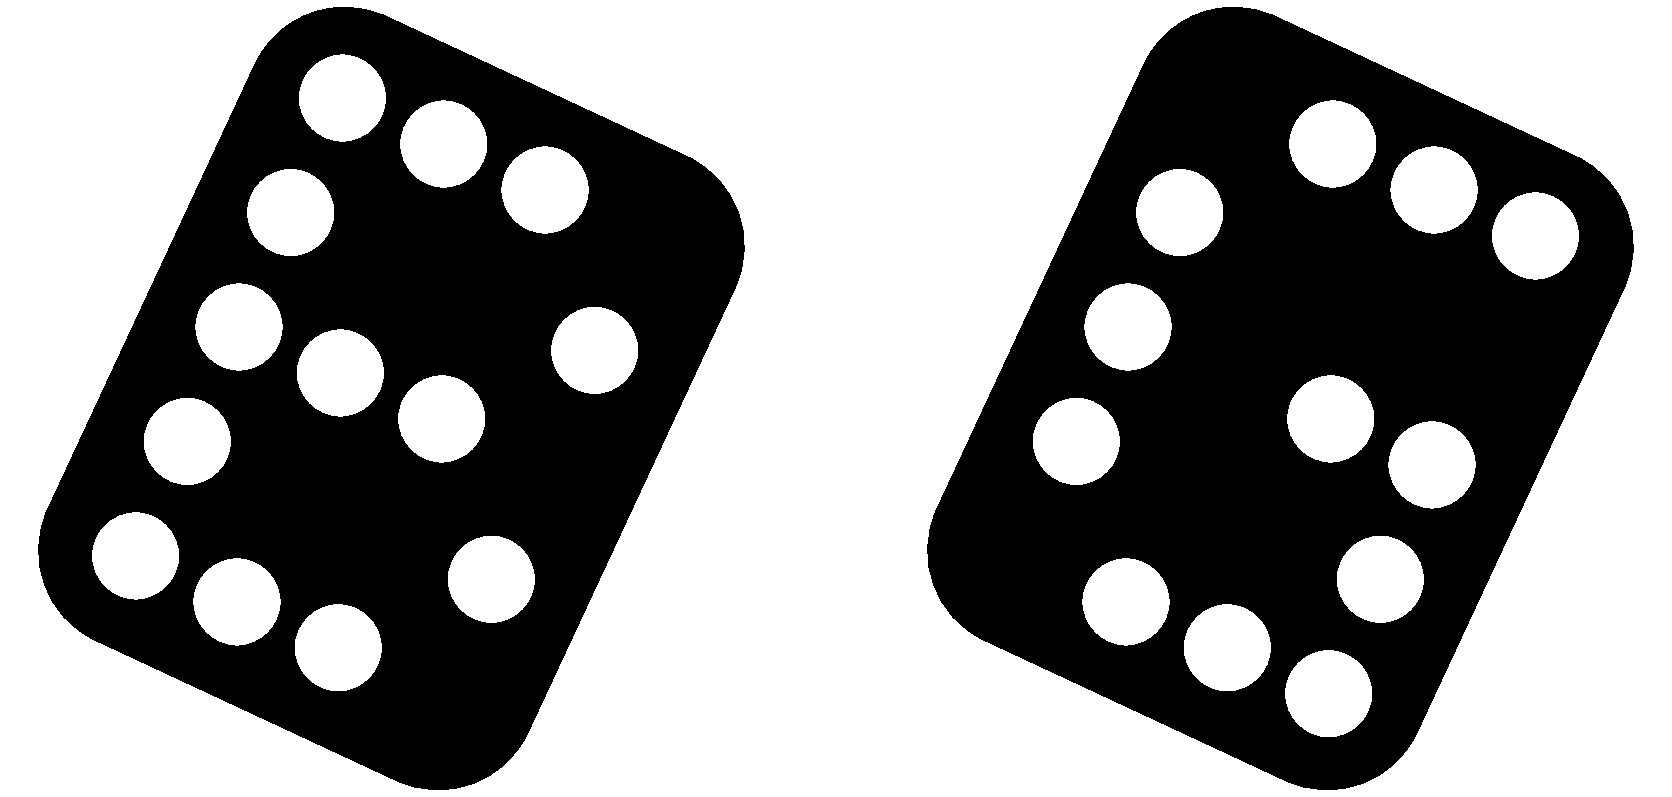
\includegraphics[height=30pt]{img/gaspedale/1.pdf}}}
	\newcommand{\pedaleRealistisch}{\raisebox{-.5ex}{
\includegraphics[height=30pt]{img/gaspedale/2.pdf}}}
	\newcommand{\tacho}{\raisebox{-.5ex}{
\includegraphics[height=30pt]{img/gaspedale/3.pdf}}}
	\newcommand{\autoPfeil}{\raisebox{-.5ex}{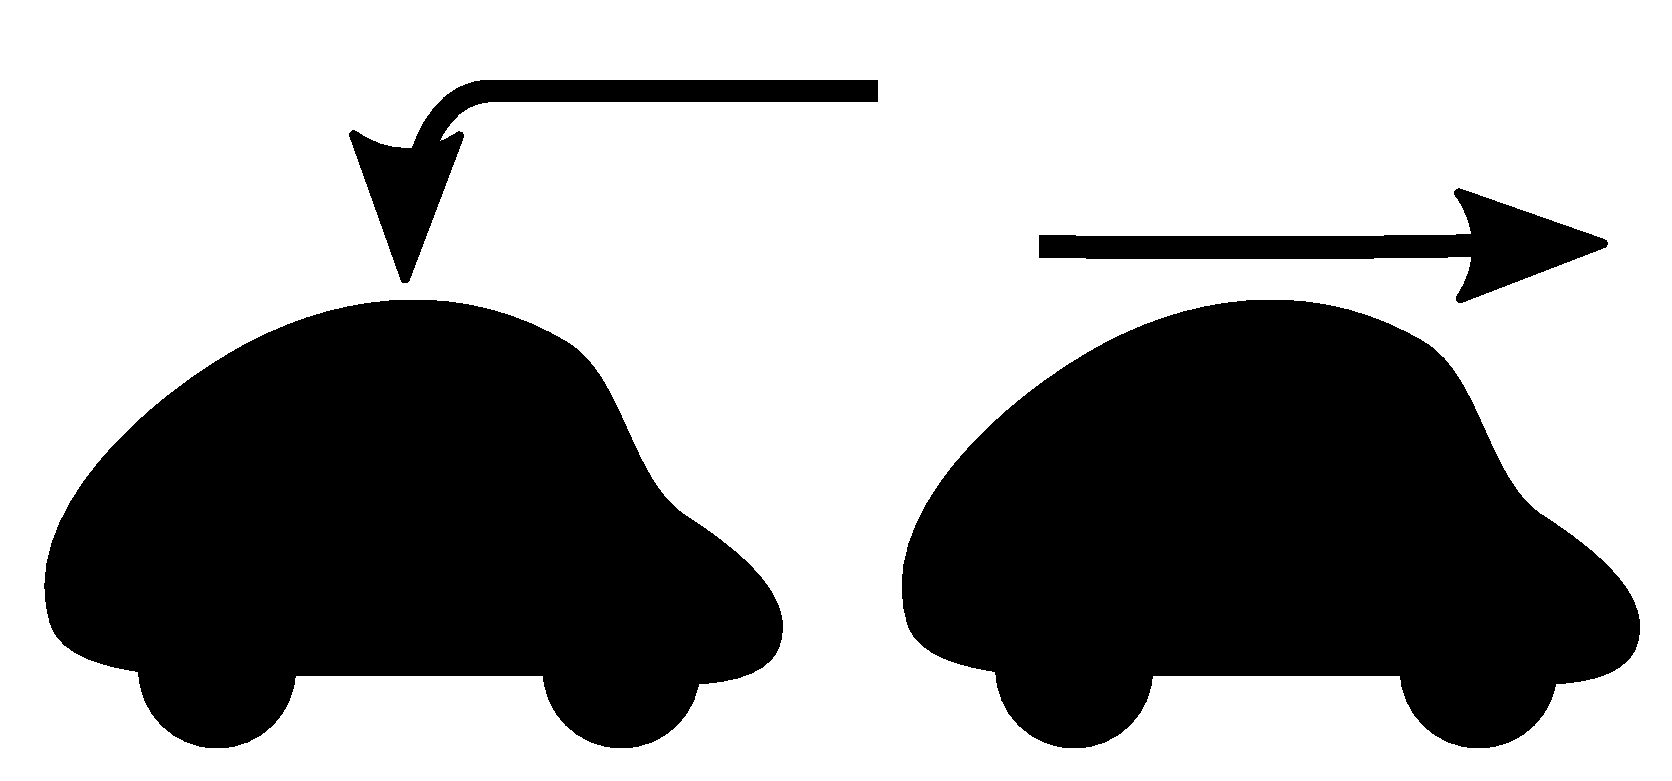
\includegraphics[height=30pt]{img/gaspedale/4.pdf}}}
	\newcommand{\symbolbild}{\raisebox{-.5ex}{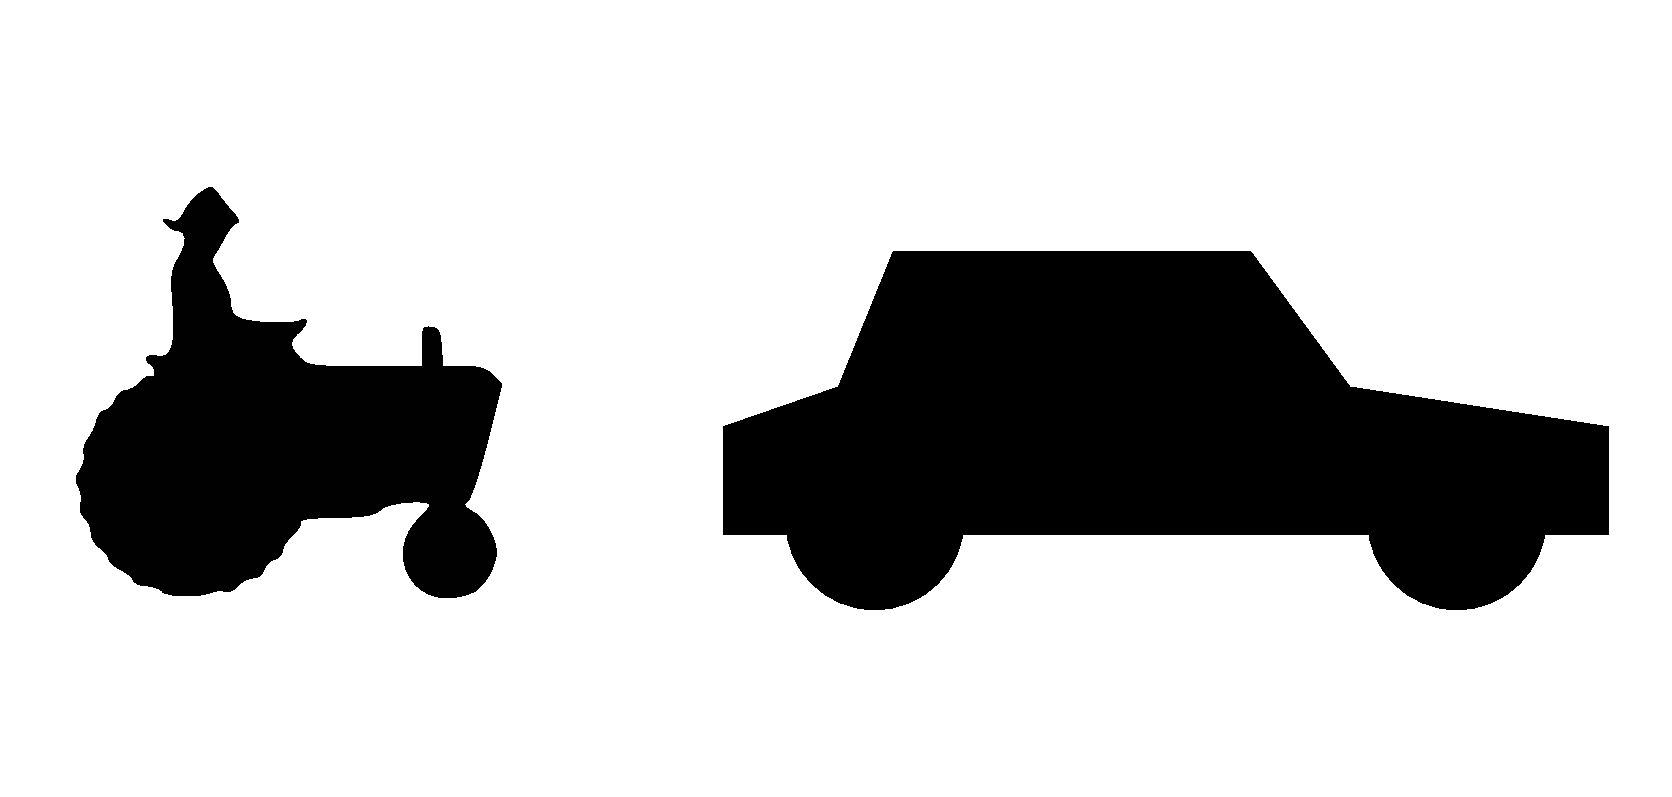
\includegraphics[height=30pt]{img/gaspedale/5.pdf}}}

	\begin{longtable}{cp{3.9cm}p{3.9cm}p{3.9cm}}%
		\toprule\label{gasevo-tabelle} \endhead%
		\bottomrule \caption{Evolution der Pedale} \endlastfoot%
			 & Beschreibung & Vorteile & Nachteile \\ \midrule
			\pedaleSchrift 		& Beschriftete Pedale werden in vielen Rennspielen verwendet. Dabei sind die Pedale mit \enquote{G} für Gas und \enquote{B} für Bremsen beschriftet. & Für deutschsprachige Spieler ist diese Einteilung einfach verständlich. & Im Rahmen der multilingualen Verwendbarkeit kann eine solche Beschriftung zu Missverständnissen führen. \\%
			\symbolbild 		& Eine weitere Möglichkeit ist die Verwendung von Symbolbildern. Dabei soll ein Symbol das langsame Fahren, und ein Symbol das schnelle Fahren symbolisieren. & Die Assoziation mit Schnell und Langsam ist sehr einfach. Die Symbole sind auch für Kinder sehr leicht verständlich. & Die Symbolbilder können nicht direkt als Schaltflächen erkannt werden. Eine Verwechslung mit beispielsweise einem Fahrzeugwechsel ist möglich und kann für Verwirrung sorgen.es wird  \\%
			\autoPfeil 			&  Die Fahrzeuge werden mit entsprechenden erklärenden Pfeilen ausgestattet. Ein Pfeil zeigt auf das Fahrzeug selbst, was einen Stillstand symbolisiert. Der zweite Pfeil zeigt vom Fahrzeug weg, was eine Beschleunigung symbolisieren soll. & Durch die Verwendung des gleichen Fahrzeugs ist eine Assoziation mit einem Fahrzeugwechsel ausgeschlossen. & Die Bedeutung der jeweiligen Pfeile ist nicht eindeutig. Ein großer Interpretationsspielraum kann sehr leicht Missverständnisse hervorrufen. \\%
			\tacho 				& Zur Symbolisierung für schnelles und langsames Fahren werden Tachos mit unterschiedlichen Nadelausschlägen verwendet. Ein voll ausgeschlagener Tacho bedeutet dabei schnelles Fahren. & Da keine irritierenden Pfeile verwendet werden, sinkt die Gefahr eines Missverständnisses. Da ebenso kein Fahrzeug symbolisiert wird, kann auch jegliches Missverständnis in dieser Richtung vermieden werden. & Tachos sind leicht verwechselbar mit einer Benzinanzeige oder einer reinen Geschwindigkeitsanzeige. Usertests haben gezeigt, das Spieler nicht intuitiv auf die Tachos drücken. \\%
			\pedaleRealistisch 	& Das finale Design geht zurück zu den Pedalen, verzichtet jedoch auf die Beschriftung. Zur besseren Unterscheidbarkeit werden unterschiedliche Designs für die jeweiligen Pedale gewählt. Dabei orientieren sich die Pedale an Pedale von realen Fahrzeugen. & Die Pedale sind einfach als Schaltflächen erkennbar, durch das Verzichten auf Beschriftung sind die Pedale multilingual einsetzbar. Durch die Orientierung an realen Pedalen ist eine Assoziation mit diesen gegeben. & Der Spieler erkennt zwar nicht auf den ersten Blick, welche Funktion die Schaltflächen haben, kann dies jedoch über \enquote{Ausprobieren} testen. \\%	
	\end{longtable}
	Der letzte Punkt im Bereich des UI Designs befasst sich mit der grundsätzlichen Positionierung der Schaltflächen und Icons. Wie in <TODO: Verlinkung zum Konzept> bereits erwähnt, soll das Spiel auf mobilen Endgeräten im Querformat gespielt und mit zwei Händen bedient werden. Da die wichtigsten Steuerelemente der Joystick sowie die Pedale sind, werden diese in den unteren Ecken zur Bedienung mit beiden Daumen positioniert. Die Schaltflächen für Pause und Zurücksetzen sind in den oberen Ecken positioniert, um eine versehentliche Betätigung durch den Spieler zu verhindern. 
	\figur{Positionierung-UI.png}{\label{ssec:ui-design}User Interface mit geöffnetem Menü}
	Die Abbildung \ref{ssec:ui-design} zeigt das User Interface, während das Menü geöffnet ist. Die Menü-Schaltflächen für \enquote{Spiel fortsetzen / Spiel starten}, \enquote{Optionsmenü öffnen} sowie \enquote{Zum Hauptmenü zurückkehren} sind an der Mitte des Bildschirms orientiert.
	\figur{Positionierung-UI-2.png}{\label{ssec:ui-design2}User Interface während des Rennens}
	Während des Spiels entspricht das User Interface der Abbildung \ref{ssec:ui-design2}. An Stelle der Schaltflächen des Menüs befinden sich am oberen Bildschirmrand nun eine Zeitanzeige, sowie eine Minikarte. Die Minikarte stellt den Streckenverlauf leicht transparent dar und zeigt die Position und Rotation des Fahrzeugs mittels eines roten Pfeils an. Die Zeitanzeige ist als Zeitstrahl dargestellt. Dabei sinkt die Größe des gelben Anteils des Zeitstrahls. Ist kein gelber Anteil mehr vorhanden, so ist die Zeit für das Rennen vollständig abgelaufen.

	\subsubsection{Physik und Steuerung}
	\subsubsection{}

\subsection{Class Diagram, DB}
\subsection{Wie wurden gewisse Dinge umgesetzt}
\subsection{Integration in Lernplattform}
s